\chapter{Introduction}

% optional if you want to include quotes; I've left the quotes I used in this template
% I showed this to my supervisor (Norm Murray) as I was writing and he laughed, so I figured it was okay ;)
\epigraph{
    ``This, recruits, is a 20 kilo ferous slug. Feel the weight! Every five seconds, the main gun of an Everest-class dreadnought accelerates one, to one-point-three percent of lightspeed. It impacts with the force a 38 kiloton bomb. That is three times the yield of the city buster dropped on Hiroshima back on Earth. That means, Sir Isacc Newton is the deadliest son-of-a-b***h in space! Now! Serviceman Burnside, what is Newton's First Law?"

    ``Sir! An object in motion stays in motion, sir!"

    ``No credit for partial answers maggot!"

    ``Sir! Unless acted on by an outside force, sir!"
    
    -- Mass Effect 2, BioWare
}

\lipsum[1]

% I've left this paragraph in to demonstrate citations and footnotes
% but also to highlight that you're allowed to be a little silly when writing your intro (presumably your main/paper chapters are written much more formally)
% at the very least, no one on my committee said I should remove them
% I had pop culture references to Sailor Moon, Mean Girls, Doctor Who, Parks and Rec, the Hamilton musical, and probably more that I'm forgetting right now
% it's your dissertation and you're allowed to let your personality come through :)

% FYI, if you find any cool old books/papers on ADS, you can probably locate them through the UofT library; the Fisher Rare Book Library might even have *original* copies!!!! but I don't think you're allowed to access them :(
The splendour of the cosmos also has an incredible capacity to ignite the imagination.
This perhaps shines brightest when it comes to works of science fiction, however.
One of the earliest works of science fiction was written by none other than Johannes Kepler himself in his post-humous work Somnium \citep{1634ssop.book.....K}, which uses a narrative about demons on the moon as a means to envision astronomical observations as viewed from the Moon.
I have conducted such work myself\footnote{Hopefully mine won't lead to my mum being arrested on suspicion of witchcraft.}, linking astronomical research and science fiction to study the dynamical stability of the numerous multi-planet systems found in BioWare's Mass Effect series \citep{2021arXiv210400175O}. 

% did you know you can write paragraphs like this in latex? I only learned about it recently and I always forget to do it. It can be really nice for editing to have each sentence on its own line in the file, though

% Modified from my dissertation intro to demo section references
To set the stage for my work in this dissertation about Cool Space Stuff, I first review some relevant background material.
I present a brief overview of what it means to be cool in Sec.~\ref{sec:intro-cool}.
In Sec.~\ref{sec:intro-space}, I give a summary of space.
Sec.~\ref{sec:intro-stuff} provides a primer of stuff.
Finally, Sec.~\ref{sec:intro-overview} gives an overview of the remaining chapters of this dissertation.

%%%%%%%%%%%%%%%%%%%%%%%%%%%%%%%%%%%%%%%%%%%%%%%%%%%%%%%%%%%%%%%%

\section{Cool}
\label{sec:intro-cool}

\lipsum[1]

% I don't feel like making example figures, so here's a real figure of mine
\begin{figure}
  \centering
  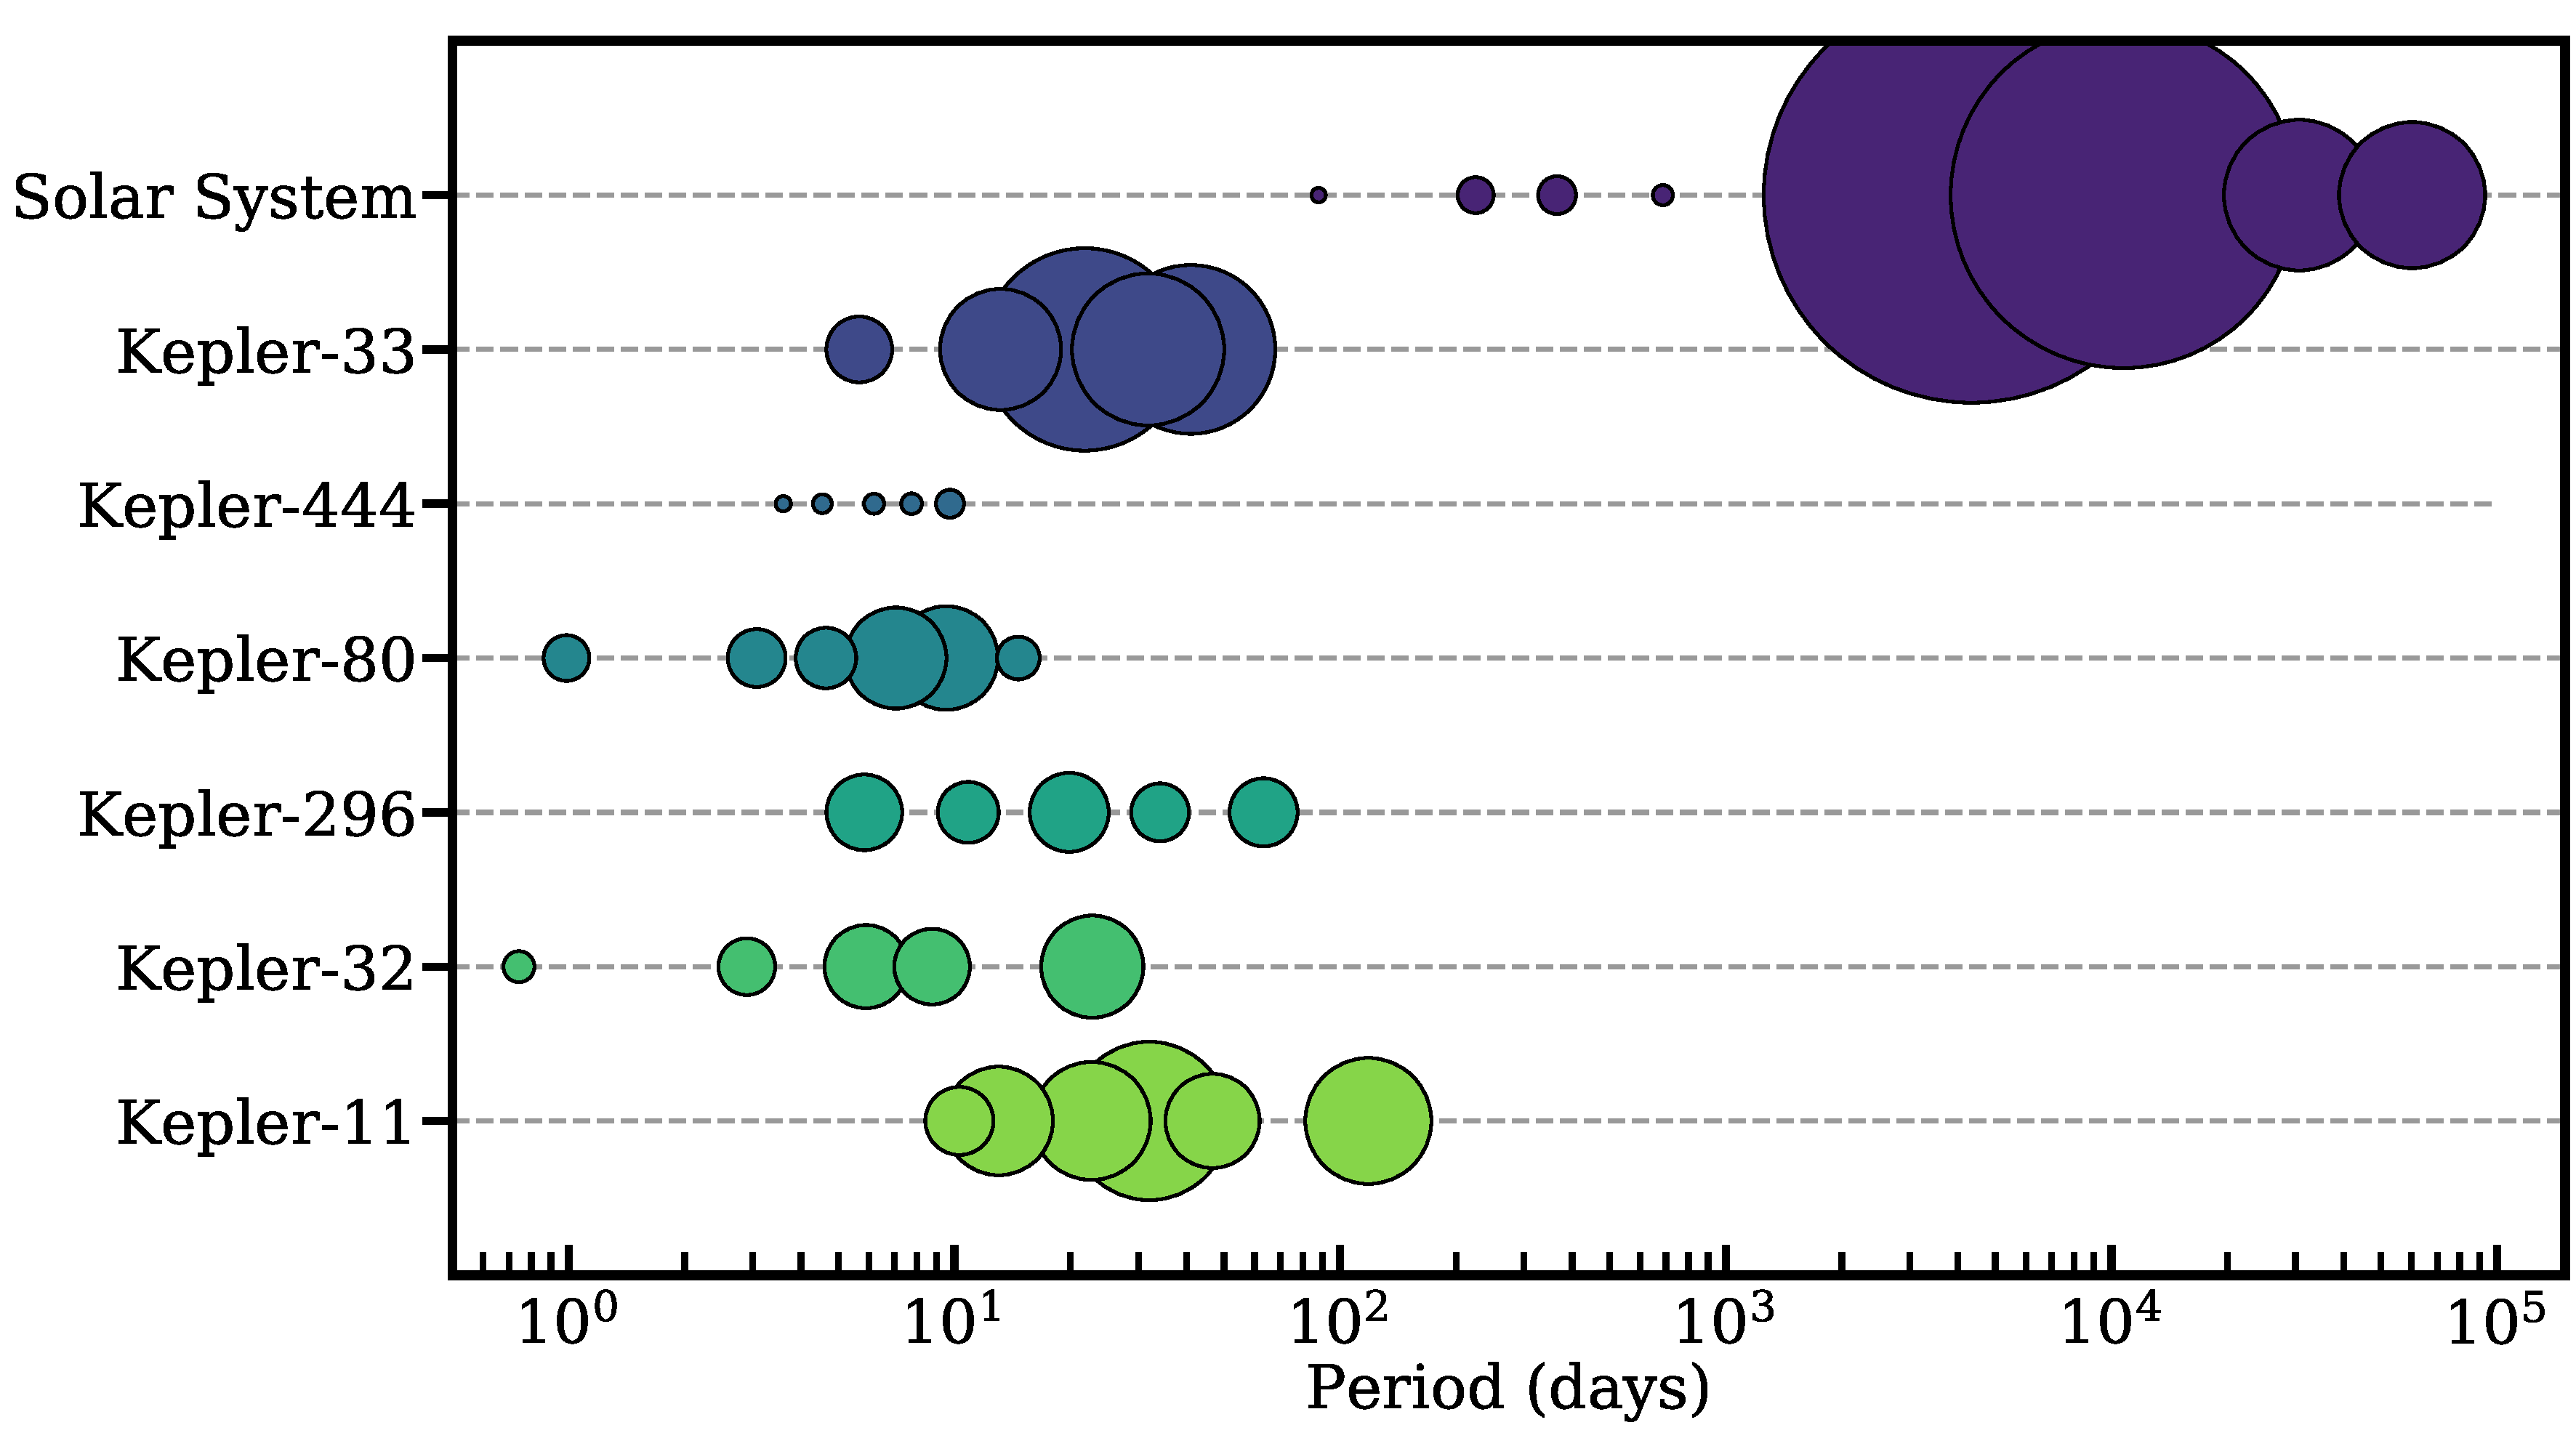
\includegraphics[width=\linewidth]{figures/intro/compact-systems-periods-feb-2019v5.pdf}
  % what's in {} is the main caption that shows up under the figure; what's in [] is the short caption for the table of contents; it's optional, but otherwise the *entire* caption shows up in the TOC and it doesn't look very nice
  \caption[Examples of cool planetary systems]{Comparison of the Solar System and several compact, multi-planet systems detected with the transit method. Each circle represents a planet, with its horizontal placement according to its orbital period and size linearly scaled according to its radius. Periods and radii are from \citep{nasa-exoplanet-archive-2019}.}
  \label{fig:cool-systems}
\end{figure}

Fig.~\ref{fig:cool-systems} shows several cool planetary systems.
Each circle represents a planet, with its horizontal placement according to its orbital period and size linearly scaled according to its radius.
Periods and radii are from \citep{nasa-exoplanet-archive-2019}.
Cool planetary systems (most of which have been detected with Kepler) have many interesting features \citep[as reviewed in e.g.][]{2021ARA&A..59..291Z,2022arXiv220310076W}.

%%%%%%%%%%%%%%%%%%%%%%%%%%%%%%%%%%%%%%%%%%%%%%%%%%%%%%%%%%%%%%%%

\section{Space}
\label{sec:intro-space}

\lipsum[4]

% I don't feel like making example table, so here's a real table of mine
\begin{table}
  \centering
  \caption[Discovery and detection counts of observed exoplanets in multi-planet systems in SPACE]{Counts of exoplanets in multi-planet systems discovered and detected (i.e. characterised) with different methods. These exoplanets are in SPACE. As of 7 April 2023, 2221 exoplanets have been discovered in 884 multi-planet systems. Values from \citet{nasa-exoplanet-archive}.}
  \begin{tabular}{rcccc}
    \toprule
    & Transit & Transit Variations & Radial Velocity & Other \\
    \midrule
    Discovered & 1645 & 24 & 506 & 46\\
    Detected & 1663 & 304 & 766 & 48\\
    \bottomrule
\end{tabular}

% 2221 planets in 884 systems
% systems counted by filtering for " b"

% detected by
% pulsar timing variations: 3
% pulsation timing variations: 0
% astrometric variations: 9
% orbital brightness modulations: 8
% microlensing: 14
% imaging: 14
% disk kinematics: 0

% eclipse timing variations: 11 
% from archive info: "Boolean flag indicating if the planet induces transit timing variations on the orbit of another another planet in the system (1=yes, 0=no)"
% how have 24 planets been detected via TTVs but only 11 induce TTVs?????
% 304 have ttv flag
% "Flag indicating if the planet orbit exhibits transit timing variations from another planet in the system (1=yes, 0=no). Note: Non-transiting planets discovered via the transit timing variations of another planet in the system will not have their TTV flag set, since they do not themselves demonstrate TTVs."
% how many total then???
% I'm confused; I've sent a message to support
  \label{tab:exoplanets-space}
\end{table}

Table~\ref{tab:exoplanets-space} shows counts for exoplanets in multi-planet systems discovered and detected in SPACE according to the NASA Exoplanet Archive's list of Confirmed Planets \citep{nasa-exoplanet-archive}.

%%%%%%%%%%%%%%%%%%%%%%%%%%%%%%%%%%%%%%%%%%%%%%%%%%%%%%%%%%%%%%%%

\section{Stuff}
\label{sec:intro-stuff}

I provide an overview of some related topic in Sec.~\ref{sec:intro-stuff-subsection}.

%%%%%%%%%%%%%%%%%%%%%%%%%%%%%%%%

\subsection[Stuff Subsection]{Stuff Subsection That's Really Long and Would Extend to Multiple Lines in the Table of Contents So You Should Probably Use a Short Title}
\label{sec:intro-stuff-subsection}

\lipsum[2]

A straight line can be described by,

\begin{equation} \label{eq:straight-line}
    y = mx + b. % lol I forgot to do this because I hate how it looks, but I think you're supposed to add a period if an equation is the end of a sentence
\end{equation} 

% I think there are other ways of doing equation labels/references in latex, but I didn't bother to look them up

In eq.~\ref{eq:straight-line}, $m$ is the slope of the line and $b$ is the y-intercept.

% this is an example of how you can reference subsubsections if you've opted not to number them (i.e. the setcounter{secnumdepth} and setcounter{tocdepth} lines are still commented out); feel free to experiment with whatever style you'd like
For more details, see~\textbf{\nameref{sec:intro-stuff-subsubsection}} in Sec.~\ref{sec:intro-stuff-subsection}.

% if setcounter{secnumdepth} and setcounter{tocdepth} lines have been uncommented, you can use this
% note that if the counter lines are still commented, the reference will provide the subsection's number (e.g. 1.3) but the hyperlink will point to the subsubsection
For more details, see~\ref{sec:intro-stuff-subsubsection}.

%%%%%%%%%%%%%%%

\subsubsection{Stuff Subsubsection}
\label{sec:intro-stuff-subsubsection}

There are ways to change the numbering of subsubsections and whether or not they appear in the table of contents, but you'll have to look that up.
I've just left the default style/formatting.

%%%%%%%%%%%%%%%%%%%%%%%%%%%%%%%%%%%%%%%%%%%%%%%%%%%%%%%%%%%%%%%%

\section{Thesis Overview}
\label{sec:intro-overview}

% this seems to be a standard way to wrap up the introduction chapter

The remainder of this dissertation describes my work towards on new Cool Space Stuff.

In Chapter~\ref{ch:paper1}, I describe my project on Cool Space Stuff that is focused on something idk \citep[published as][]{2017Icar..293...52O}.

In Chapter~\ref{ch:paper2}, I describe my project on some different Cool Space Stuff.  \citep[publication accepted; preprint posted as][]{2023arXiv230612967O}.

Finally, I summarise the findings and conclusions of these two projects in Chapter~\ref{ch:conclusions} and discuss my results within the broader context of the field of Cool Space Stuff. I finish by describing exciting new prospects for gaining new and critical insight into Cool Space Stuff.